\chapter{Introduction}
\label{ch:introduction}
Inferix is a decentralized GPU network for visual computing and AI, it is built to bridge the needs of users and hardware owners. Its solution meets real-world problems across a range of industries, not only for the AI field but also for high-quality rendering needs. Users (e.g.~3D graphics artists, game developers, enterprises) who need GPU computing power for rendering high-quality graphics can use Inferix system to continuously access these precious resources with faster processing time and more efficient spending.
\begin{figure}[h]
    \centering
    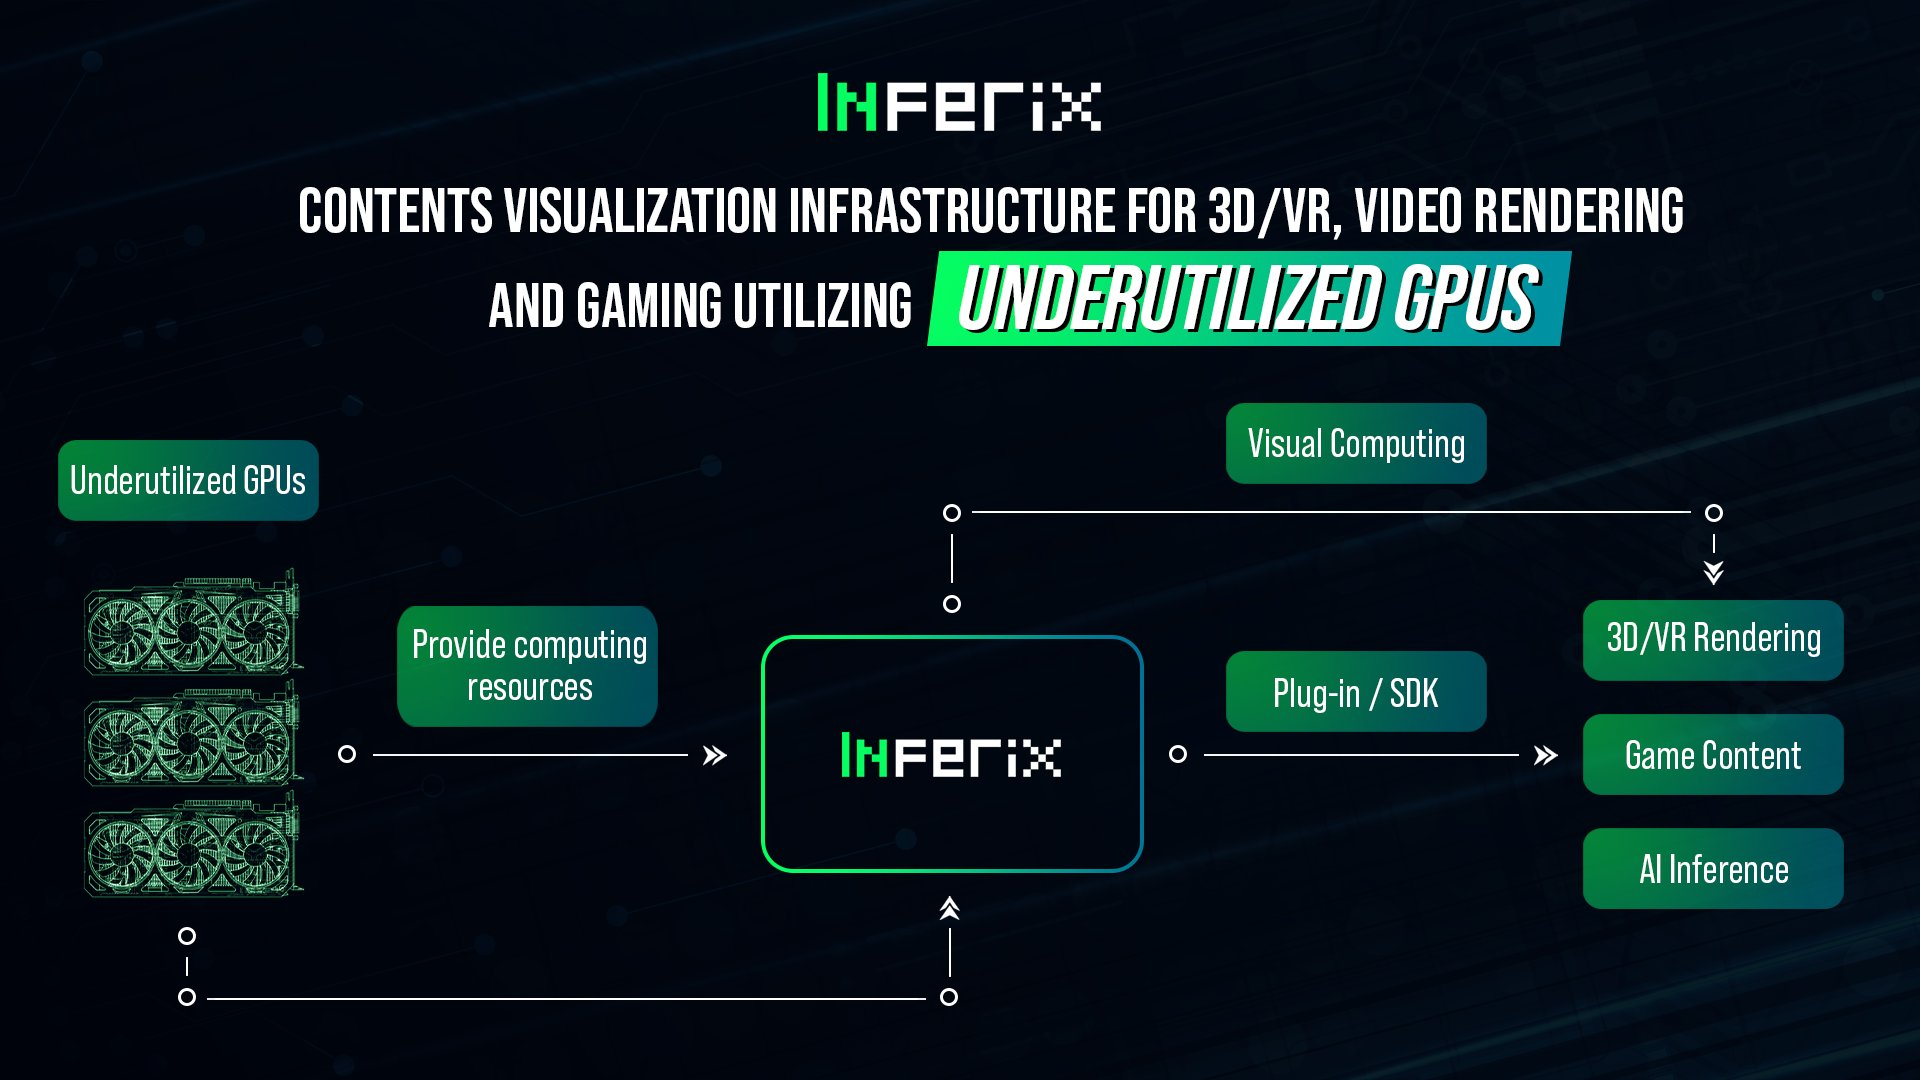
\includegraphics[width=0.8\textwidth]{inferix_high_level_architecture.jpg}
    \caption{High level architecture}
    \label{fig:inferix_rendering_network_high_level}
\end{figure}
Owners of GPUs can share idle resources to Inferix network and earn long-term passive income while simultaneously balancing their main jobs or leisure activities.

In this document, we briefly present first the graphics rendering network of Inferix, then focus on the internal details of the verification procedure for rendered images.


% Inferix provides a decentralized 3D graphics rendering service: remote people can submit Blender graphics scenes then receive rendered images and videos, others can join the service to let their computing resources for hire. Since the graphic rendering processes are intensively resources (GPU, RAM, disk storage, etc.) consuming and not everyone possessing these resources, Inferix regulates this exigence by in the one hand helping artists get their jobs done without equipping very high-end workstations. In the other hand, it allows individuals making profit from their unused high-performance computation resources.


\section[Rendering network]{Rendering network}
The graphics rendering service consists in a network of decentralized machines called \emph{nodes} which are of $3$ kinds: \emph{manager}, \emph{worker} and \emph{verifier}. The \emph{managers} and \emph{verifiers} are dedicated machines of Inferix while the \emph{workers} are machines joined by GPU owners. The number of \emph{workers} is normally much larger than the number of \emph{managers} and \emph{verifiers}.
\begin{figure}[h]
    \centering
    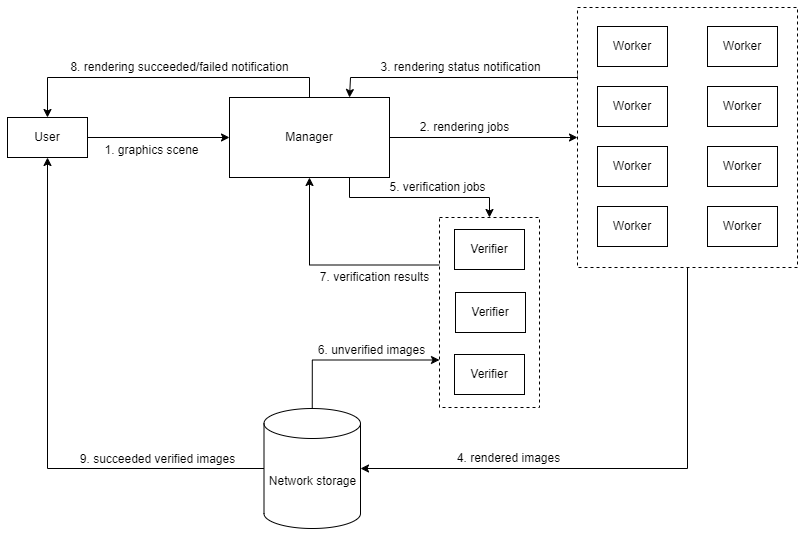
\includegraphics[width=0.8\textwidth]{rendering_service.png}
    \caption[Graphics rendering flow]{Graphics rendering flow}
    \label{fig:rendering_service}
\end{figure}
A typical rendering session contains several steps which are shown in~\autoref{fig:rendering_service}:
\begin{enumerate}
    \item A user submits a graphics scene to some \emph{manager} using the Inferix plugin for client.
    \item The \emph{manager} who receives the graphics scene builds corresponding rendering jobs, each job consists of several parameters: range of images to be rendered, image format, etc. These job will be dispatched to \emph{workers}.
    % Then it pushes the jobs into a job queue. The \emph{manager} maintains also a pool for registered \emph{workers} and \emph{verifiers}, rendering jobs from the job queue are dispatched to the pooled workers.
    % it dispatches jobs from the job queue to workers in the pool.
    \item Receiving a rendering job, a \emph{worker} renders the graphics scene using the parameters given by the job. When it finishes, it sends the rendered images to a shared storage.
    \item The \emph{worker} then notifies a \emph{manager} about the status of rendering job.
    \item The notified manager creates a verification job and dispatches this job to some \emph{verifier}.
    % consisting of several parameters: range of images to be verified, image format, etc. Then it pushes the job into a job queue. 
    \item Receiving a verification job, a \emph{verifier} checks the authenticity of the corresponding rendered images.
    \item The \emph{verifier} then notifies the \emph{manager} about the verification results.
    \item The \emph{manager} notifies the user about the graphics rendering result.
    \item If there is no error, the user can finally download the rendered images/video from the shared storage.
\end{enumerate}
%  directly using the Inferix plugin for Blender (or via some Web interface!?). The \emph{manager} creates a job corresponding to this graphics scene, queues this job into a pool then dispatches to \emph{workers} which do the rendering. The rendered images will be sent back from \emph{workers} to several \emph{verifiers} which check if the images are valid. The validity is notified to the \emph{manager} to accept or reject the rendered results: a job is considered valid only if all results of this job pass the verification, in this case the results will be sent back to users.
% (...add a figure here describing the high-level architect of rendering service)
The \emph{managers} synchronize a database of rendering and verification jobs. That makes the rendering service  being both logically and physically decentralized: a graphic scene can be simultaneously rendered by different \emph{workers} and later checked by different \emph{verifiers}, the machines of \emph{workers} and \emph{verifiers} can be also located at different geographical locations.

\section[Rendering output verification]{Rendering output verification}\label{sec:output_verification}
One of the most important problems that Inferix has to solve is to maintain the \emph{authenticity} of rendered result. That means how to warranty that once a user submits a valid graphics scene, then after waiting for an amount of time, the user will receive an authentically rendered result. The authenticity can be defined informally as the result received from the rendering network and the result received if the scene is rendered by the genuine graphics rendering software are human perceptual indistinguishable.

However, the \emph{workers} joined the rendering network are mostly workstations\footnote{Except the dedicated machines of Inferix.} of GPU owners who want to make profit from their unused computing resources. Respecting the privacy of GPU owners, beside a lightweight open source software client installed to manage the communication with the network, there is completely no control on \emph{workers}.




% There is no control (except initial hardware requirements to join the network!?) over these machines, so the graphics rendering is proceeded without being controlled. In order to guarantee that the graphics scenes are correctly rendered, we propose a mechanism called \emph{Active Noise Generation and Verification} which is presented in detail in~\autoref{ch:scene_watermarking}.

% (...add a concrete example about an attack)